
\newcommand{\rcpsp}{RCPSP} %{Resource-Constrained Project Scheduling}
\newcommand{\Wsh}{W_k}
\newcommand{\estm}{ES}
\newcommand{\letm}{LC}

\ChapterAuthor[
Constraint Programming formulations and propagation algorithms]{
Constraint Programming formulations and propagation algorithms}{
Philippe \Name{Laborie} \and Wim \Name{Nuijten}}
\label{cp-formulations-and-filtering}

This chapter presents the classical representation of \rcpsp\ in
Constraint-Based Scheduling as well as the propagation algorithms for
temporal constraints and resource capacity constraints (time-tabling,
disjunctive reasoning, edge-finding, energetic reasoning, precedence
energy, and balance constraint) used to solve the \rcpsp\ through Constraint-Based Scheduling.

\section{Constraint formulations}

\subsection{Constraint Programming}

Constraint Programming (CP) is based on a declarative description of
a problem as (1) a set of decision variables with domains, i.e., sets of
possible values, for instance the start time of an activity with its
possible time windows; and (2) a set of constraints restricting the
combinations of values the decision variables can take, for instance a
precedence constraint between the end time of activity A and the start time of
activity B.
	
Constraints can be defined either explicitly as a set of compatible tuples of variable assignments or implicitly, for instance through an algebraic relation (e.g. $x\neq y$). A solution to a CP problem is a complete assignment of the variables satisfying all the constraints.

The search for a solution usually explores a search tree whose branches correspond to decisions (for instance instantiating a variable $x$ to a given value $v$). During the search, constraints are used actively to remove inconsistent values from the current domain of variables. This process is known as {\bf constraint propagation} \cite{Bessiere2006}. One way of propagating constraints consists in enforcing arc-consistency. A constraint is said to be arc-consistent if the domains of its variables have been reduced so that they only contain values that are supported by at least one solution to the constraint. For instance if the domain of variables $x$ and $y$ in constraint $C=(x \leq y)$ are so that $x \in [5,10]$ and $y \in [0,7]$, enforcing arc-consistency on $C$ will reduce these domains to $x \in [5,7]$ and $y \in [5,7]$. At each node explored by the search, constraints are propagated until the fix point of the propagation is reached. 

A particularly important class of constraints are the so called {\bf global constraints}. Such constraints represent a set of basic constraints (for instance $alldifferent(x_1,...,x_n)$ standing for $\forall i \in [1,n], j \in [i+1,n], x_i \neq x_j$). Algorithms for propagating global constraints are able to propagate from a global point of view in an efficient way. The typical scheduling example of such a global constraint is the constraint that propagates on the combination of all activities requiring capacity from a non-renewable resource.

\subsection{Constraint-Based Scheduling}

Constraint-Based Scheduling is the discipline that studies how to
solve scheduling problems by using CP. It has over the years grown
into one of the most successful application areas of
CP. Constraint-Based Scheduling extends CP by providing constructs
such as activities and resources which have a scheduling semantics. An
activity usually corresponds to at least 3 decision variables: start
time, end time and processing time or duration. The domains of these
variables represent the possible time windows and duration of the
activity. Classical constraints in Constraint-Based Scheduling are
temporal constraints between activities and resource capacity constraints. Different types of resources can be modeled \cite{Baptiste2006}: unary resources, cumulative resources, producible/consumable resources, state resources, etc. Resource demands represent a certain demand of resource (this quantity can be a decision variable) for a given activity. Although most of all the extensions described in Part II of this book can be modeled and solved using the paradigm of Constraint-Based Scheduling, we focus in this chapter on the basic formulation of \rcpsp\ and the underlying constraint propagation algorithms. More detailed surveys of constraint propagation algorithms for Constraint-Based Scheduling are available in \cite{dorndorf99,BLPNbook01}.

The basic \rcpsp\ can be formulated as shown in Table \ref{table:RCPSPModel} in a Constraint-Based Scheduling approach using the Optimization Programming Language (OPL) \cite{VanHentenryck99}. The precedence graph structure is defined at line {\tt 8} as a set of precedence arcs {\tt {i,j}}. The set of activities is defined at line {\tt 11}, activity {\tt A[i]} being constructed with duration {\tt p[i]}. An additional activity of duration {\tt 0} representing the makespan is defined at line {\tt 12}. The set of cumulative resources is created at line {\tt 13}, resource {\tt R[k]} being of capacity {\tt B[k]}. Discrete resources post a global capacity constraint on the set of activities that require the resource. The objective function (minimize end time of makespan activity) is specified at line {\tt 14} followed by the constraints of the problem. Each activity {\tt A[i]} is constrained to finish before the makespan activity (line {\tt 17}) and to require {\tt b[i][k]} units of resource {\tt R[k]} at line {\tt 19}. Finally, the precedence constraints of the precedence graph {\tt G} are posted at line {\tt 22}. 

\begin{table}[!hbp]
\begin{verbatim}
 1  // Data
 2  struct Precedence { int i; int j; }; 
 3  int q            = ...; // Number of resources
 4  int n            = ...; // Number of activities
 5  int p[1..n]      = ...; // Processing times
 6  int B[1..q]      = ...; // Resource capacities
 7  int b[1..n,1..q] = ...; // Resource requirements
 8  {Precedence} G   = ...; // Precedence graph
 9
10  // Model
11  Activity A[i in 1..n](p[i]);
12  Activity makespan(0);
13  DiscreteResource R[k in 1..q](B[k]);
14  minimize makespan.end
15  subject to { 
16    forall(i in 1..n) {
17      A[i] precedes makespan;
18      forall(k in 1..q : 0 < b[i][k])
19        A[i] requires(b[i][k]) R[k];
20    };
21    forall(<i,j> in G)
22      A[i] precedes A[j];
23  };
\end{verbatim}
\normalsize
\label{table:RCPSPModel}
\caption{An OPL model of the basic \rcpsp}
\end{table}

The next section describes the principles of the classical algorithms for propagating temporal constraints (subsection \ref{tempct}) and resource constraints (subsections \ref{timetabling}-\ref{balance}).

\section{Constraint propagation algorithms}

\subsection{Temporal constraints}
\label{tempct}

Temporal relations between activities can be expressed by linear constraints
between start and end variables of activities. For instance, a
standard precedence constraint between two activities $A_i$ and $A_j$
stating that $A_j$ is to be started after $A_i$ has ended can be
modeled by the linear constraint $C_i \le S_j$. In
the general case of \rcpsp\ with time lags, with both $x$ and $y$ a start or end variable and $\delta$ an
integer, temporal relations can be expressed by constraints of the
type $x - y \leq \delta$.

When the temporal constraint network is sparse, as it is usually the
case in \rcpsp, such constraints can be easily propagated using a
standard arc-consistency algorithm \cite{Lhomme93}. In addition, 
a variant of Ford's algorithm (see for instance \cite{Gondran84}) proposed 
by Cesta and Oddi \cite{CestaOddi96} can be used to detect any inconsistency 
between such constraints, in time polynomial to the number of constraints and
independent of the domain sizes.

When the temporal network is dense or when it is useful to compute and
maintain the minimal and maximal delay between any pair of time points
in the schedule, path consistency can be enforced on the network \cite{DechterMeiri91} for
example by applying Floyd-Warshall's All-Pairs-Shortest-Path algorithm
\cite{Floyd62}. 

\subsection{Timetabling}
\label{timetabling}

Timetabling relies on the computation of the minimal resource usage by
the current activities in the schedule at every date $t$ 
\cite{lepape94}. This aggregated demand profile is maintained  during 
the search. It  allows restricting the domains of the start and end times 
of activities by removing the dates that would lead to an over-consumption of the resource.

Suppose that activity $A_i$ requires $b_{ik} \in
[b^{-}_{ik},b^{+}_{ik}]$ units of resource $R_k$ and is such that
$LS_i<EC_i$. Then we know that $A_i$ will surely execute over the time
interval $[LS_i,EC_i)$ requiring at least $b^{-}_{ik}$ units of
$R_k$. See activity $A_1$ in Figure \ref{fig:Laborie:Timetabling} for
an illustration. The minimal contribution of activity $A_i$ at time
$t$ is thus given by the function:

\vspace*{-5mm}
\begin{eqnarray*}
  U_k(A_i,t) & = & 
   \left\{
   \begin{array}{ll}
   b^{-}_{ik}  & \textrm{if $LS_i \leq t < EC_i$}\\
   $0$  & \textrm{otherwise}
   \end{array}
   \right.
   \nonumber
\end{eqnarray*}

For each  resource $R_k$, a curve $U_k(t)$ is maintained that aggregates all 
these demands: $U_k(t) = \sum_{i=1}^{n}  U_k(A_i,t)$.

\begin{Figure}[!htbp] { Timetabling }
\includegraphics[angle=270,width=10cm]{LaborieNuijtenCP/Laborie-Timetabling.eps}
%\caption{Timetabling}
\vspace*{-15mm}
\label{fig:Laborie:Timetabling}
\end{Figure}

It is clear that if there exists  a  date $t$  such that  $U_k(t)$ is
strictly greater than the maximal capacity of the resource $B_k$, the
current  schedule  cannot lead to a solution and the search  must
backtrack.   

Furthermore, $U_k(t)-U_k(A_i,t)$ represents the requirement by all
activities but $A_i$ on $R_k$ at date $t$. If there exists a date $t$
such that $U_k(t)-U_k(A_i,t)+b^{-}_{ik}>B_k$, then activity $A_i$
cannot be executing at time $t$. In particular, if the above relation
is true for some $t$ with $ES_i \leq t < EC_i$ (resp. $LS_i \leq t <
LC_i$), it allows to increase (resp. decrease) the earliest start time
(resp. latest completion time) of activity $A_i$ until the first date
$t'$ such that $U_k(t')-U_k(A_i,t')+b^{-}_{ik} \leq B_k$. Similar
reasoning can be applied to find new upper bounds on the quantity of
resource required by activities. The main advantage of the timetabling technique
is its low practical algorithmic complexity which is linear or even sub-linear in the number of activities. For this reason, it is the main technique used today for scheduling renewable resources on large problems.

\subsection{Disjunctive reasoning}
\label{sec:CP:disjreas}
Let $A_i$ and $A_j$ be two activities  on a resource $R_k$ such that $b^-_{ik} + b^-_{jk} > B_k$.  
As such they cannot overlap in time and thus either $A_i$ precedes $A_j$ or $A_j$ precedes
$A_i$, {\em i.e.}, the disjunctive constraint holds between these activities. In general the disjunctive constraint achieves arc-consistency on the formula:

\[ [b_{ik} + b_{jk} \le B_k] \vee [C_i \le S_j] \vee [C_j \le S_i] \]

The disjunctive constraint can be propagated on all activities with a worst case complexity in $O(n\log n)$ \cite{Vilim2004}.

\subsection{Edge-finding}
\label{CP:edgeFinding}
Let $\phi \subset {\mathcal A}$ a subset of activities that require a given resource $R_k$ of capacity $B_k$ and $A_i \in {\mathcal A}\setminus \phi$. Let's denote: 
\begin{itemize}
\item $ES_{\phi}=\min_{A_j \in \phi}{ES_j}$, the earliest start time of all activities in $\phi$
\item $EC_{\phi}=\min_{A_j \in \phi}{EC_j}$, the earliest completion time of all activities in $\phi$
\item $LC_{\phi}=\max_{A_j \in \phi}{LC_j}$, the latest completion time of all activities in $\phi$
\item $W_{\phi}=\sum_{A_j\in \phi}{p_j \cdot b_{jk}}$, the global energy required by $\phi$. 
\end{itemize}

The basic idea of edge-finding and activity interval techniques is to ensure that for any subset of activities $\phi$, resource $R_k$ provides enough energy over the time interval $[ES_{\phi},LC_{\phi})$ to allow the execution of all the activities of $\phi$, that is: $W_{\phi} \leq B_k\cdot(LC_{\phi}-ES_{\phi})$. Constraint propagation is usually performed by applying the three following deduction rules:

\begin{enumerate}

\item If $B_k\cdot (LC_{\phi} - ES_{\phi \cup \{i\}}) < W_{\phi \cup \{A_i\}}$, then $A_i$ must finish after all activities in $\phi$, in particular $EC_i := max (EC_i, EC_{\phi})$.

\item If $ES_{\phi} < ES_i < EC_{\phi}$ and $B_k \cdot (LC_{\phi} - ES_{\phi}) < W_{\phi} + b_{ik} \cdot (min(LC_{\phi}, EC_i)-ES_i)$, then at least one activity $A_j$ in $\phi$ must precede $A_i$ as otherwise, $A_i$ would start between $ES_{\phi}$ and $EC_{\phi}$ and there would not be enough energy to execute $\phi \cup \{A_i\}$ between $ES_{\phi}$ and $LC_{\phi}$ thus $ES_i := max(ES_i, EC_{\phi})$.
	
\item If $ES_i < ES_{\phi} < EC_i$ and $B_k \cdot (LC_{\phi} - ES_{\phi}) < W_{\phi}+ b_{ik} \cdot (EC_i-ES_{\phi})$, then  $A_i$ must finish after all activities in $\phi$, in particular $EC_i := max (EC_i, EC_{\phi})$.
\end{enumerate}

These rules allows to update the earliest start or completion times of activities and symmetrical rules allow to update the latest start and completion times. Edge finding (\cite{Nuijten94}) and activity intervals propagation (\cite{Caseau1996}) are very similar techniques that mainly differ in the way the propagation rules are triggered: edge-finding algorithms are global algorithms that perform all updates on a given resource whereas activity interval approaches are performed incrementally as soon as the time bound of a activity changes.

Note that specific edge-finding algorithms have been designed for the special case of disjunctive resources ($B_k=1$) \cite{BLPNbook01}. These algorithms can be implemented with a time complexity in $O(n \log n)$ \cite{Vilim2004}.

\subsection{Energy reasoning}
\label{subsec:CuSPEner}
Energy based constraint propagation algorithms compare the amount of
energy provided by a resource over some interval $[t_1, t_2)$ to the
amount of energy required by activities that have to be processed over this
interval. \cite{ErschlerLopez91} proposes the following  definition of the required energy consumption that
takes into account the fact that activities cannot be interrupted. 
Given a resource $R_k$, an activity $A_i$ and a time interval $[t_1, t_2), \Wsh(A_i, t_1, t_2)$,
the ``Left-Shift / Right-Shift'' required energy consumption of resource $R_k$ by activity $A_i$
over $[t_1, t_2)$ is $b_{ik}$ times the minimum of the three following
durations.
\begin{itemize}
\item the length of the interval: $t_2 - t_1$;
\item the number of time units during which $A_i$ executes after time $t_1$ if $A_i$ is left-shifted, {\em i.e.}, scheduled as soon as possible: $p_i^{L}(t_1) = \max(0, p_i - \max(0, t_1 - \estm_i))$; 
\item the number of time units during which $A_i$ executes before time $t_2$ if $A_i$ is right-shifted, {\em i.e.}, scheduled as late as possible: $p_i^{R}(t_2) = \max(0, p_i - \max(0, \letm_i - t_2))$.  
\end{itemize}
This leads to
$\Wsh(A_i, t_1, t_2) = b_{ik} \cdot \min(t_2 - t_1, p_i^{L}(t_1), p_i^{R}(t_2))$. 

The Left-Shift / Right-Shift overall required energy consumption
$\Wsh(t_1, t_2)$ over an interval $[t_1, t_2)$ is then defined as the
sum over all activities $A_i$ of $\Wsh(A_i, t_1, t_2)$. 

It is obvious that if there is a feasible schedule then $B_k \cdot (t_2 - t_1) - \Wsh(t_1, t_2) \ge 0$ for all $t_1$ and $t_2$ such that $t_2 \ge t_1$.

It is shown in \cite{BaptisteLePape01} how the values of $\Wsh$ can be
used to adjust activity time bounds. Given an activity $A_i$ and a
time interval $[t_1, t_2)$ with $t_2 < \letm_i$, it is examined
whether $A_i$ can end before $t_2$.  If there is a time interval
$[t_1, t_2)$ such that
$$
\Wsh(t_1, t_2) - \Wsh(A_i, t_1, t_2) + b_{ik} \cdot p_i^{L}(t_1) > B_k \cdot (t_2 - t_1)
$$
then a valid lower bound of the end time of $A_i$ is
$$
t_2 + \frac{1}{b_{ik}}(\Wsh(t_1, t_2) - \Wsh(A_i, t_1, t_2) + b_{ik} \cdot p_i^{L}(t_1) - B_k \cdot (t_2 - t_1))
$$
Similarly, when
$$
\Wsh(t_1, t_2) - \Wsh(A_i, t_1, t_2) + b_{ik} \cdot \min(t_2 - t_1, p_i^{L}(t_1)) > B_k \cdot (t_2 - t_1),
$$
$A_i$ cannot start before $t_1$ and a valid
lower bound of the start time of $A_i$ is
$$
t_2 - \frac{1}{b_{ik}}(C (t_2 - t_1) - \Wsh(t_1, t_2) + \Wsh(A_i, t_1,t_2)).
$$

\cite{BaptisteLePape01} presents a $O(n^3)$ algorithm to compute 
these time bound adjustments for all $n$ activities. It is first shown
there are $O(n^2)$ intervals $[t_1, t_2)$ of interest. Given an
interval and an activity, the adjustment procedure runs in $O(1)$. As
such the obvious overall complexity of the algorithm is thus
$O(n^3)$. An interesting open question is whether there is a quadratic
algorithm to compute all the adjustments on the $O(n^2)$ intervals
under consideration. Another open question at this point is whether
the characterization of the $O(n^2)$ time intervals in
\cite{BaptisteLePape01} can be sharpened in order to eliminate some
intervals and reduce the practical complexity of the corresponding
algorithm. Finally, it seems reasonable to think that the time bound
adjustments could be sharpened. Even though the energy tests can be
limited (without any loss) to a given set of intervals, it could be
that the corresponding adjustment rules cannot.


\subsection{Precedence graph}

The constraint propagation algorithms above reason on the absolute position of activities in time (through their time bounds $ES_i$, $EC_i$, $LS_i$, $LC_i$). They provide an efficient propagation when these time bounds are tight but the propagation becomes weaker when time window of activities is large. 

Some additional propagation algorithms have been designed that reason on the relative position of activities on resources (precedence relations in a precedence graph) rather than their absolute position only. As a consequence, these algorithms allow a much stronger propagation when the time windows of activities are large and when the current schedule contains many precedence relations as it is usually the case in \rcpsp. These algorithms require that a temporal network representing the relations between the time-points of all activities (start and end) using the point algebra of (\cite{VilainKautz86}) is maintained during the search. We denote $\{\emptyset, \prec, \preceq, =, \succ, \succeq, \neq, ? \}$ the set of qualitative relations between the time points of the schedule $S_i$, $C_i$. The temporal network is in charge of maintaining the transitive closure of those relations. Let $r$ be one of the above relations, we denote $\neg (x\ r\ y)$ if and only if the relation $x\ r\ y$ cannot be deduced from the network.

The initial set of relations consist of the precedences $S_i\prec C_i$ for each activity $A_i$ and $C_i \preceq S_j$ for each precedence constraint of the problem. During the search additional precedence relation can be added as decisions or as the result of constraint propagation.

Figure \ref{fig:Laborie:PrecGraph} illustrates an example of such a precedence graph. An arrow between two time-points $x$ and $y$ means $x \prec y$. Once the transitive closure of the graph has been computed, the following relations hold: $S_3 \prec C_2$, $\neg (S_1 \prec C_4)$.

\begin{Figure}[!htbp] { Precedence graph }
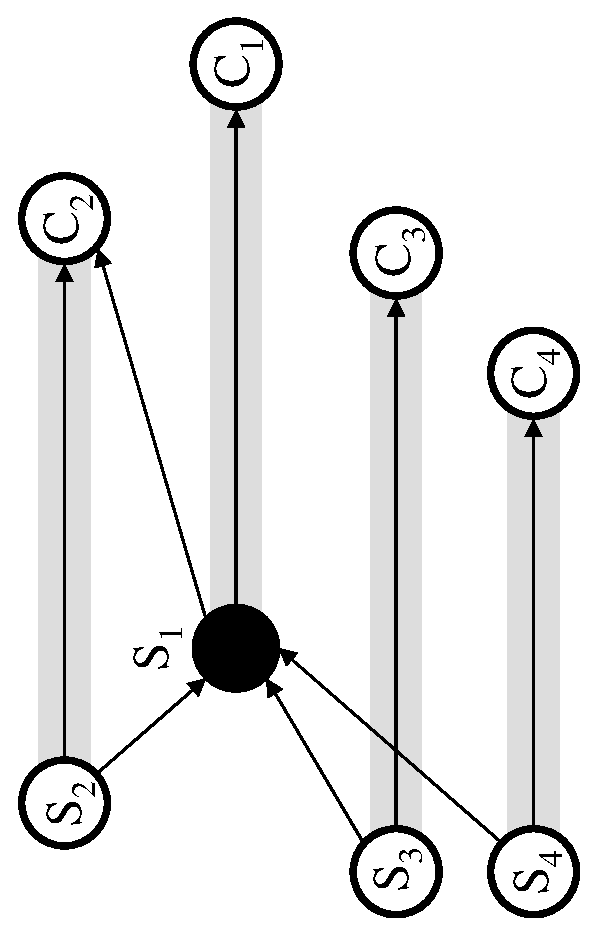
\includegraphics[angle=270,width=5cm]{LaborieNuijtenCP/Laborie-Balance.eps}
\label{fig:Laborie:PrecGraph}
\end{Figure}

\subsection{Energy precedence}

The {\em energy precedence} propagation algorithm (\cite{Laborie03a}) for an activity $A_i$ on a resource $R_k$ ensures that for each subset $\Omega$ of predecessor activities of activity $A_i$ the resource provides enough energy to execute all activities in $\Omega$ between $ES_\Omega$ and $S_i$. More formally, if $ES_\Omega = \min_{A_j \in \Omega} ES_j$ and $W_{\Omega,k} = \sum_{A_j \in \Omega} p_j \cdot b_{ik}$, it performs the following deduction rule:
\[\forall \Omega \subset \{ A_j \in {\mathcal A}, C_j \preceq S_i\}, ES_i := max(ES_i, ES_\Omega+ \lceil W_{\Omega,k}/B_k \rceil ) \]

The propagation of the energy precedence constraint can be performed for all the activities $A_i$ on a resource and for all the subsets $\Omega$ with  a total worst-case  time complexity of $O(n (p+log(n))$ where $n$ is  the number  of activities  on  the resource and $p$  the maximal number  of predecessors of a  given  activity in the temporal network ($p < n$). 

\subsection{Balance constraint}
\label{balance}

On a renewable resource, the {\em balance constraint} (\cite{Laborie03a}) can be defined as follows. 
The basic idea  of the algorithm is to compute, for each activity $A_i$ on a resource $R_k$, a lower bound on the resource usage at the start time of $A_i$ (a symmetrical reasoning can be applied to perform some propagation based on a lower bound on the resource usage at the completion time of $A_i$). Using the temporal network a lower bound  on the resource utilization at date  $S_i+\epsilon$ just after the start time of $A_i$ can be computed assuming that all the resource requirements that do not necessarily overlap $S_i$ will not overlap it:
\[L_k(i) = \sum_{j / (S_j\preceq S_i) \land (C_j\succ S_i)} b_{jk} \]
Given this bound, the balance constraint is able to discover three types  of information:

\textbf{Dead ends}.  Whenever $L_k(i)>B_k$, the  resource will  surely  be over-consumed just
after time-point $S_i$ so the search has reached a dead end.

\textbf{New bounds on time variables}. If $L_K(i) \leq B_k$, $\Delta(i)=B_k-L_K(i)$ represents a slack of capacity that must not be exceeded by all the resource requirements that, currently, do not necessarily overlap $S_i$ but could overlap it. Let $P(i)=\{A_j / (S_j\preceq S_i) \land \lnot (C_j \succ S_i) \}$. We suppose the activities $(A_{j_1},\cdots,A_{j_u},\cdots,A_{j_p})$ in $P(i)$ are ordered by decreasing earliest completion time $EC_j$. Let $v$ be  the index  in $[1,p]$ such that:
\[\sum_{u=1}^{v-1} b_{j_uk} \le \Delta(x) < \sum_{u=1}^{v}b_{j_uk}\]
If event $S_i$ is executed at a date $S_i< EC_{j_v}$, not enough activities of $P(i)$ will be  able to be completed strictly before $S_i$ in order  to ensure the resource is not over-consumed just after $S_i$ as in this case, the consumed quantity will be at least $L_K(i)+\sum_{u=1}^{v}b_{j_uk}>B_k$.  Thus, $EC_{j_v}$ is a valid  lower  bound of $S_i$. 

\textbf{New precedence relations}. Suppose there exists activity $A_y$ in $P(i)$ such that:
\[\sum_{A_z \in P(i), C_z \succeq C_y} b_{zk} > \Delta(x)\]
Then, if we had  $S_i\prec C_y$, we would see  that again there is  no way to avoid a resource over-consumption as it would consume at least:

\[L_k(i)+\sum_{A_z \in P(i), C_z \succeq C_y} b_{zk}  > B_k\]

Thus, the necessary precedence relation: $C_y \preceq S_i$ can be deduced and added to the current temporal network. 

On the precedence graph of Figure \ref{fig:Laborie:PrecGraph}, if all activities require 1 unit of the same resource $R_k$ of capacity $3$, the balance constraint applied at time-point $S_1$ would compute $L_k(1)=b_{1k}+b_{2k}=2$ and deduce that $\min(EC_3,EC_4)\leq S_1$.

The balance algorithm can be executed for all the activities $A_i$ with a global worst-case complexity in $O(n^2)$ if the propagation that discovers new precedence relations is not turned on, in $O(n^3)$ for a full propagation. In practice, there are many ways to shortcut this worst case and in particular, it was noticed that the algorithmic cost of the extra-propagation that discovers new precedence relations was in general negligible.   

\section{Conclusion}

Constraint-Based Scheduling provides a wide spectrum of propagation algorithms for renewable resources ranging from sub-linear to quadratic time complexities. The selection of a combination of propagation algorithms clearly depends on the size of the problem being solved. 

For small problems until a few tens of renewable resources and a few hundred activities on each resource, a strong propagation scheme may be used. This is for instance the case of the MCS method described in section \ref{comp:results} and experimented on small RCPSPs. It uses a combination of timetabling, disjunctive, edge-finding, energy precedence and balance constraints. 

Larger problems are generally solved using meta-heuristics. These methods, for instance the LNS described in section \ref{comp:results}, are usually less sensitive to constraint propagation than tree search methods and light propagation schemes can be used, typically, only using timetabling.

